\chapter{Architectures of Database Systems}

\section{Model Types}

\begin{center}
	\begin{tikzpicture}[
	every node/.style={rectangle, draw, fill=blue!20, minimum width=2.5cm, minimum height=1cm, align=center},
	node distance=1.5cm and 1.5cm
	]
	
	% Hierarchical model
	\node (root) at (0,0) {Root};
	\node (child1) [below left=of root] {Child 1};
	\node (child2) [below=of root] {Child 2};
	\node (child3) [below right=of root] {Child 3};
	
	\draw (root) -- (child1);
	\draw (root) -- (child2);
	\draw (root) -- (child3);
	
	% Network model
	% Shift down a bit for separation
	\node (n1) at (-2.5,-5) {Node 1};
	\node (n2) at (2.5,-5) {Node 2};
	\node (n3) at (-1.5,-7) {Node 3};
	\node (n4) at (1.5,-7) {Node 4};
	
	\draw (n1) -- (n2);
	\draw (n1) -- (n3);
	\draw (n2) -- (n4);
	\draw (n3) -- (n4);
	
\end{tikzpicture}

\end{center}

\subsection{Hierarchical Model}
\begin{itemize}
	\item Tree-like structure with one parent per child
	\item Good performance for one-to-many relationships, but poor flexibility
	\item each record has only one parent record
	\item a record is a collection of fields where each filed contains one value
	\item the fields of a record are defined by its type
	\item used only in few database systems today, e.g. in IBM Information management System
\end{itemize}

\subsection{Network Model}
\begin{itemize}
	\item Allows many-to-many relationships with interconnected nodes
	\item More flexible than hierarchical models but more complex to manage
	\item most general form of a data structure $\rightarrow$ No limitation to the links between records
	\item enables complex data structures but only simple operations
	\item widely replaced by the relational model
\end{itemize}

\subsection{Relational Model}
\begin{itemize}
	\item Data is stored in tables with rows (records) and columns (fields)
	\item Uses primary and foreign keys to establish relationships between tables
	\item created to be simple 
	\item became more popular than the network model with increased computing power
	\item postulates independence of the language and implementation
	\item originally implementations of the relational model were too slow for productive use, but with growing computing power the relational model became the standard abstraction model for database systems
	\item declarative queries, the use of values, and set orientation make it easy to use compared to the network model which uses pointers and is record oriented
\end{itemize}

\section{Building Relational Database Systems}
\subsection{Monolithic Approach}
\begin{enumerate}
	\item \textbf{Single Codebase}: All components-query processor, storage manager, transaction manager, etc. -reside in one codebase
	\item \textbf{Tight coupling}: Components depend heavily on each other, making it hard to change one without affecting other
	\item \textbf{Centralized control}: All functionality is in one process, internal calls are fast (no network latency)
	\item \textbf{Difficult Maintenance \& Scalability}: Updating or scaling individual components is harder than in modular systems
\end{enumerate}

\begin{figure}[H]
	\centering
	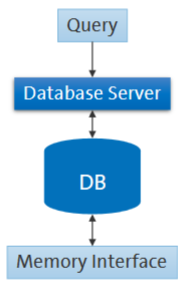
\includegraphics[width=0.2\linewidth]{media/architectures/monolithicApproach}
	\caption[Monolithic Approach]{Monolithic Approach}
	\label{fig:monolithicapproach}
\end{figure}

\subsection{The 5 Layer Model}

\begin{enumerate}
	\item \textbf{Data System Layer}
	\begin{itemize}
		\item SQL parsing, query planning, optimization, execution
		\item semantic understanding of data (tables, schemas)
		\item \textbf{Output}: A logical query execution plan
		\item \textbf{Manages}: Relations, views indexes
	\end{itemize}
	\item \textbf{Access System Layer}: 
	\begin{itemize}
		\item Logical access to data: retrieval and update
		\item navigation, use of logical pointers and index structures
		\item manages record format and system catalogs
	\end{itemize}
	\item \textbf{Storage System Layer}: 
	\begin{itemize}
		\item Physical data organization on disk
		\item record management, free space access paths
		\item manages tress, hash structures
	\end{itemize}
	\item \textbf{Buffer \& File System Layer}: 
	\begin{itemize}
		\item Manages in memory-pages
		\item page replacement strategies
		\item interacts with file system and hardware
		\item handles logging and recovery and durability
	\end{itemize}
\end{enumerate}

\section{Record management}
\begin{itemize}
	\item Records stored on fixed-length pages (records can vary in length)
	\item Addressing via Tuple Identifier (TID) = Page ID, Index in Page
	\item Heap Management: Keeps track of free space for placing new records
\end{itemize}

\section{Organization of Pages}
\begin{itemize}
	\item Pages linked in doubly-linked list
	\item Each page contains: Header info (page ID; previous/next page), Metadata (free space, record type)
	\item Pages support efficient access and stable record addressing even during data migration
\end{itemize}

\section{Tuple Identifier ( TIDs)}
\begin{itemize}
	\item stable address of a record
	\item record updates: 
	\begin{itemize}
		\item if too large: Moved to another page, old page stores pointer
		\item if small: reorganized in place no change to TID
	\end{itemize}
	\item ensures address consistency even after migration or deletion
\end{itemize}

\section{Use of Indexes}
\begin{itemize}
	\item prevent full scans $\rightarrow$ use indexes for faster access
	\item Types of access: 
	\begin{itemize}
		\item Sequential scan
		\item sorted access
		\item direct (by key)
		\item Navigational (related records)
	\end{itemize}
	\item Requirements: Fast, direct, topology-preserving access	
\end{itemize}

\section{B-Tree and Index Classification}
\begin{itemize}
	\item Indexes are classified based on:
	\begin{itemize}
		\item \textbf{Primary or Secondary}: based on uniqueness
		\item \textbf{Simple or Multilevel}: one-level or hierarchical indexing
	\end{itemize}
	\item Storage Structures:
	\begin{itemize}
		\item Tree-structured: e.g., B-Tree
		\item Sequential: e.g., sorted lists
		\item Scattered: e.g., hash tables
	\end{itemize}
	\item Access Methods:
	\begin{itemize}
		\item Key comparison: e.g., B-Trees
		\item Key transformation: e.g., hashing
	\end{itemize}
	\item B-Tree features:
	\begin{itemize}
		\item Reduces disk accesses by organizing keys hierarchically
		\item Dynamic reorganization through page splits and merges
		\item Supports direct access and range queries
	\end{itemize}
\end{itemize}

\section{Creating Indexes in SQL}
\begin{itemize}
	\item Syntax examples:
	\begin{itemize}
		\item \texttt{CREATE INDEX my\_index ON myTable(myAttr);}
		\item \texttt{CREATE UNIQUE INDEX my\_index ON myTable(myAttr);}
		\item \texttt{CREATE INDEX my\_index ON myTable(a + b * (c - 1), a, b);}
	\end{itemize}
	\item Special options:
	\begin{itemize}
		\item \texttt{INCLUDE}: add attributes to leaf nodes only
		\item \texttt{[DIS]ALLOW REVERSE SCANS}: control scan direction
	\end{itemize}
	\item Attribute order in composite indexes matters:
	\begin{itemize}
		\item Index on (A, B) can be used for queries on A or A+B, not just B
	\end{itemize}
	\item Not all features available in every DBMS $\rightarrow$ always check system documentation
\end{itemize}

